
% JuliaCon proceedings template
\documentclass{juliacon}
\setcounter{page}{1}

\begin{document}

% **************GENERATED FILE, DO NOT EDIT**************

\title{TSML (Time Series Machine Learning)}

\author{Paulito P. Palmes}
\author{Joern Ploennigs}
\author{Niall Brady}
\affil{IBM Dublin Research Lab}

\keywords{Julia, Time Series, Machine Learning, Filters, Feature Extraction, Classification, Prediction, Aggregation, Imputation}



\maketitle

\begin{abstract}

  Over the past years, the industrial sector has seen many innovations brought about by automation. 
  Inherent in this automation is the installation of sensor networks for status monitoring and data collection. 
  One of the major challenges in these data-rich environments is how to extract and exploit information from 
  these large volume of data to detect anomalies, discover patterns to reduce downtimes and manufacturing 
  errors, reduce energy usage, predict faults/failures, effective maintenance schedules, etc. 
  To address these issues, we developed TSML. Its technology is based 
  on using the pipeline of lightweight filters as building blocks to process huge amount of industrial time series data in parallel.  

\end{abstract}

\section{Introduction}

\textbf{TSML} is a Julia\cite{bezanson2017julia} package for time series data processing, classification, and prediction. 
It provides common API for ML libraries from Python's ScikitLearn, 
R's caret, and native Julia MLs for seamless integration of heterogeneous 
libraries to create complex ensembles for robust time-series prediction, clustering, and classification.
TSML has the following features:
\begin{enumerate}
\item data type clustering/classification for automatic data discovery
\item aggregation based on date/time interval
\item imputation based on symmetric Nearest Neighbors
\item statistical metrics for data quality assessment and classification input features
\item ML wrapper with more than 100+ libraries from caret, scikitlearn, and julia
\item date/value matrix conversion of 1-D time series using sliding windows to generate features for ML prediction
\item pipeline API for high-level description of the processing workflow
\item specific cleaning/normalization workflow based on data type
\item automatic selection of optimised ML model
\item automatic segmentation of time-series data into matrix form for ML training and prediction 
\item extensible architecture using just two main interfaces: fit and transform
\item meta-ensembles for automatic feature and model selection
\item support for distributed computation for scalability and speed
\end{enumerate}

The \textbf{TSML} package assumes a two-column input composed of \emph{dates} and \emph{values}. 
The first part of the workflow aggregates values based on the specified date/time 
interval which minimizes occurrence of missing values and noise. The aggregated 
data is then left-joined to the complete sequence of dates in a specified date/time interval. 
Remaining missing values are replaced by \textit{k} nearest neighbors where \textit{k} is the symmetric 
distance from the location of missing value. This approach can be called several 
times until there are no more missing values.

For prediction tasks, TSML extracts the date features and 
convert the value column into matrix form parameterized by 
the size and stride of the sliding window. The final part joins
 the date features and the value matrix to serve as input to the 
 ML with the output representing the values of the time periods 
 to be predicted ahead of time.
 
\textbf{TSML} uses a pipeline which iteratively calls the \emph{fit} and \emph{transform}
families of functions relying on `multiple dispatch` to select the correct 
algorithm from the steps outlined above. Machine learning functions in 
\textbf{TSML} are wrappers to the corresponding Scikit-learn, Caret, and native Julia ML libraries. 
There are more than hundred classifiers and regression functions available using a common API.

\section{TSML Workflow}
\label{sec:tsmlworkflow}
%
 Did
\textbf{TSML} workflow borrows the idea of Unix pipeline\cite{orchestra2014, combineml2016}.
The main elements in a pipeline are series of filters
each performing one specific task and does it well. 

\vskip 6pt
To illustrate, below describes the main steps in using \textbf{TSML}.
First, we create filters for csv reading, aggregation, imputation, data quality
assessment.

\begin{lstlisting}[language = Julia]
fname = joinpath(dirname(pathof(TSML)),
  "../data/testdata.csv")
csvfilter = CSVDateValReader(Dict(
  :filename=>fname,
  :dateformat=>"dd/mm/yyyy HH:MM"))
valgator = DateValgator(Dict(
  :dateinterval=>Dates.Hour(1)))
valputer = DateValNNer(Dict(
  :dateinterval=>Dates.Hour(1)))
stfier = Statifier(Dict(:processmissing=>true))
\end{lstlisting}

We can then setup a pipeline containing these filters to process the csv data
by aggregating the time series hourly and check the data quality using the
\emph{Statifier} filter.

\begin{lstlisting}[language = Julia]
apipeline = Pipeline(Dict(
  :transformers => [csvfilter, valgator, stfier]))
fit!(apipeline)
mystats = transform!(apipeline)
@show mystats
\end{lstlisting}

\begin{figure}[htbp]
   \centering
   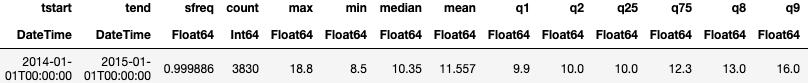
\includegraphics[width=\columnwidth]{stat1.png} % requires the graphicx package
   \vskip 2pt
      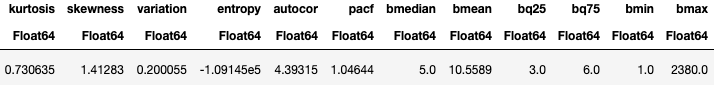
\includegraphics[width=\columnwidth]{stat2.png} % requires the graphicx package
   \caption{Data Quality Statistics. Column names starting with `b` refer to statistics of contiguous blocks of missing data.}
   \label{fig:dataquality}
\end{figure}

Calling the \emph{fit} and \emph{transform} in the pipeline
iteratively calls the corresponding \emph{fit} and \emph{transform} within each filter. 
This common API relying on Julia's multi-dispatch mechanism greatly simplifies the implementations, operations, 
and understanding of the entire workflow. In addition, extending TSML functionality is just a 
matter of creating a new data type filter and define its own  \emph{fit} and \emph{transform} 
functions.

\vskip 3pt

In the \emph{Statifier} filter result, blocks of missing data is indicated by column names starting
with \emph{b}. Running the code above indicates that there are plenty of missing data blocks.
We can add the \emph{ValNNer} filter to perform \emph{k} nearest neighbour imputation and check
the statistics:

\begin{lstlisting}[language = Julia]
bpipeline = Pipeline(Dict(
  :transformers => [csvfilter, valgator, 
                    valputer,stfier]))
fit!(bpipeline)
imputed = transform!(bpipeline)
@show imputed
\end{lstlisting}

\begin{figure}[htbp]
   \centering
   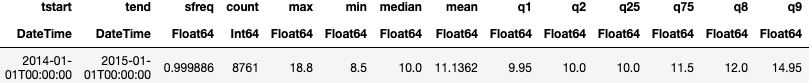
\includegraphics[width=\columnwidth]{imputed1.png} % requires the graphicx package
   \vskip 2pt
      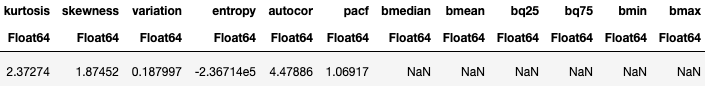
\includegraphics[width=\columnwidth]{imputed2.png} % requires the graphicx package
   \caption{Statistics after Imputation. All statistics for blocks of missing data indicate NaN to indicate the stats of empty set. This implies that all missing blocks are imputed.}
   \label{fig:imputation}
\end{figure}

The result in Fig.~\ref{fig:imputation} now indicates \emph{NaN} for all missing data statistics column because the set 
of missing blocks count is now empty.

\vskip 3pt

We can also visualise our time series data using the \emph{plotter} filter instead of the \emph{statifier} as shown in Fig~\ref{fig:mplot}. Looking closely, you will see discontinuities in the plot due to blocks of missing data.

\begin{lstlisting}[language = Julia]
pltr=Plotter(Dict(:interactive => true))
plpipeline = Pipeline(Dict(
  :transformers => [csvfilter, valgator, pltr]))
fit!(plpipeline)
transform!(plpipeline)
\end{lstlisting}

\begin{figure}[htbp]
   \centering
   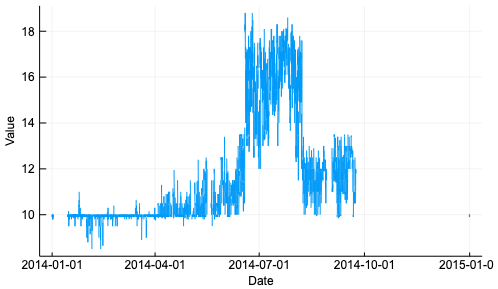
\includegraphics[width=\columnwidth]{mplot.png} % requires the graphicx package
   \caption{Plot with Missing Data}
   \label{fig:mplot}
\end{figure}

Using the imputation pipeline described before, we can visualise the result of imputation by replacing the \emph{Statifier} with the \emph{Plotter} filter. Figure~\ref{fig:amplot} shows the plot after imputation which gets rid of missing data.

\begin{lstlisting}[language = Julia]
bplpipeline = Pipeline(Dict(
  :transformers => [csvfilter, valgator, 
                    valputer,pltr]))
fit!(bplpipeline)
transform!(bplpipeline)
\end{lstlisting}

\begin{figure}[htbp]
   \centering
   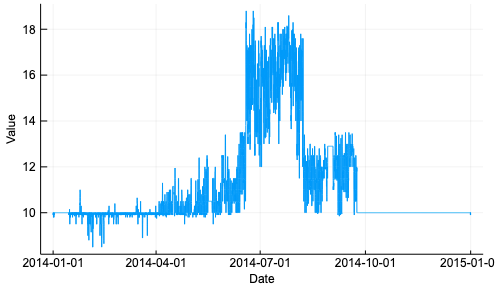
\includegraphics[width=\columnwidth]{amplot.png} % requires the graphicx package
   \caption{Plot after Data Imputation}
   \label{fig:amplot}
\end{figure}

\subsection{Processing Monotonic Time Series}
In this section, we will show additional filters we use to handle monotonic data which are commonly used in energy/water meter sensors as well as in footfall sensors. In the former case, the time series type is strictly monotonically increasing while in the latter case, the monotonicity happens daily by resetting the sensor to certain baseline. We use the filter called \emph{Monotonicer} which automatically detects the two types of monotonic sensors and apply the normalisation accordingly. 

\begin{lstlisting}[language = Julia]
mono = joinpath(dirname(pathof(TSML)),
  "../data/typedetection/monotonic.csv")
monocsv = CSVDateValReader(Dict(
  :filename=>mono,
  :dateformat=>"dd/mm/yyyy HH:MM"))
\end{lstlisting}

Let us plot the monotonic data with the usual workflow of aggregating and imputing the data first.

\begin{lstlisting}[language = Julia]
monopipeline = Pipeline(Dict(
  :transformers => [monofilecsv,valgator,
                    valputer,pltr]))
fit!(monopipeline)
transform!(monopipeline)
\end{lstlisting}

\begin{figure}[htbp]
   \centering
   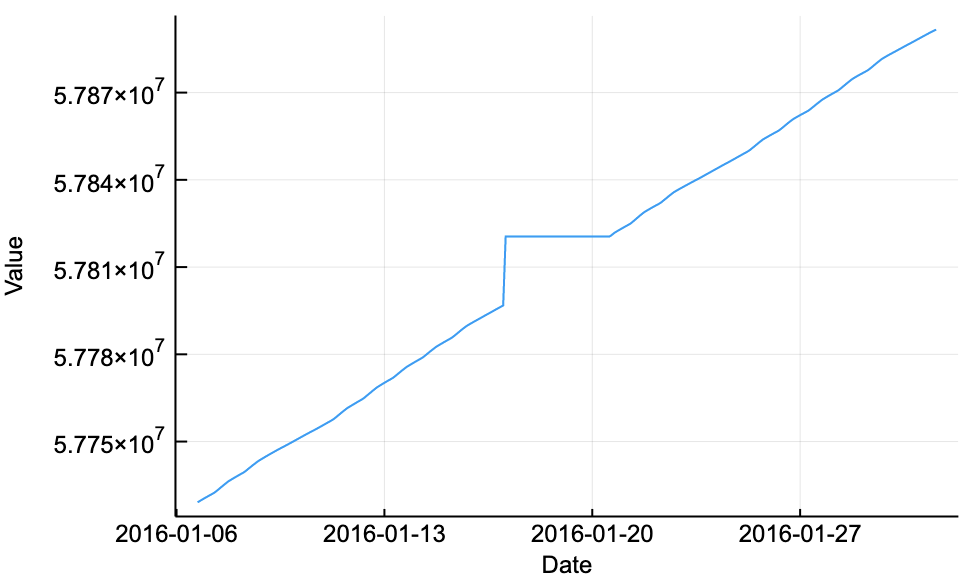
\includegraphics[width=0.9\columnwidth]{mono.png} % requires the graphicx package
   \caption{Monotonic Time Series}
   \label{fig:mono}
\end{figure}

Let us now normalise the data by adding the \emph{Monotonicer} filter in the pipeline and plot.
\begin{lstlisting}[language = Julia]
mononicer = Monotonicer(Dict())
monopipeline = Pipeline(Dict(
  :transformers => [monofilecsv,valgator,valputer,
                    mononicer, pltr]))
fit!(monopipeline) 
transform!(monopipeline)
\end{lstlisting}

\begin{figure}[htbp]
   \centering
   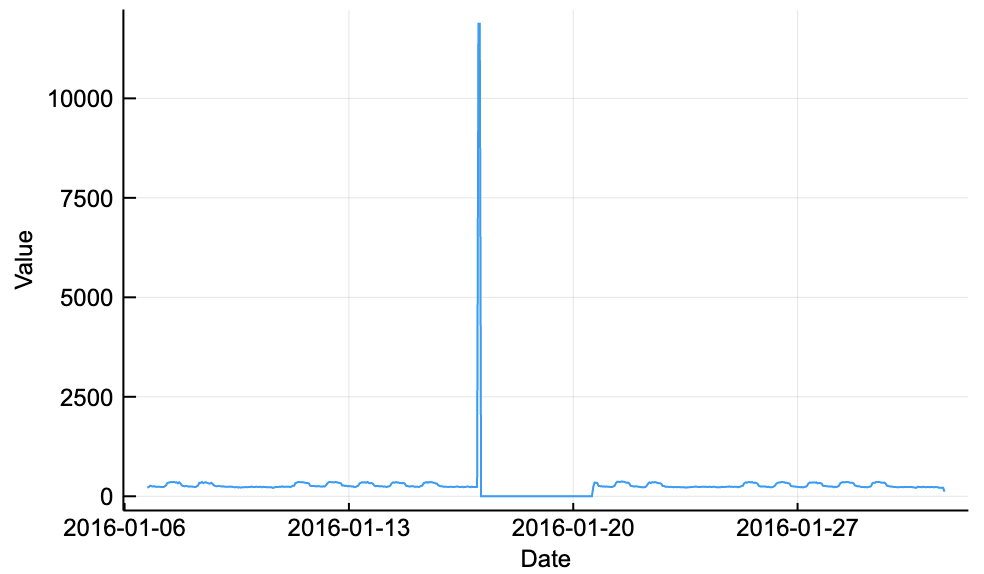
\includegraphics[width=\columnwidth]{mononicer.png} % requires the graphicx package
   \caption{Normalized Monotonic Time Series}
   \label{fig:nmono}
\end{figure}

The presence of outlierdue to some random errors during meter reading  becomes obvious after the normalisation. To remedy this issue, we can add the \emph{Outliernicer} filter which detects outliers and replace them using similar KNN imputation technique used by the \emph{DateValNNer} filter.

\begin{lstlisting}[language = Julia]
outliernicer = Outliernicer(
       Dict(:dateinterval=>Dates.Hour(1)))
monopipeline = Pipeline(Dict(
  :transformers => [monofilecsv,valgator,valputer,
                    mononicer,outliernicer,pltr]))
fit!(monopipeline)
transform!(monopipeline)
\end{lstlisting}

\begin{figure}[htbp]
   \centering
   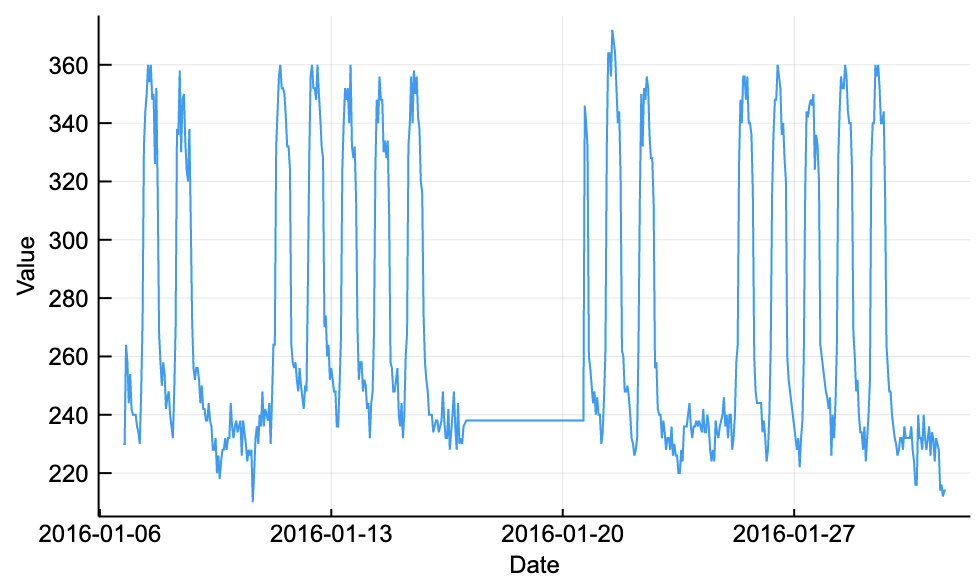
\includegraphics[width=\columnwidth]{outnicer.png} % requires the graphicx package
   \caption{Normalized Monotonic Time Series With Outlier Removal Filter}
   \label{fig:outnicer}
\end{figure}

\subsection{Processing Daily Monotonic Time Series}
We follow similar workflow in the previous subsection to normalize daily monotonic time series. We visualise first the original data, apply the \emph{Monotonicer} and \emph{Outliernicer} filters, and plot the cleaned data to make sure monotonicity is gone.

\begin{lstlisting}[language = Julia]
dailymono = joinpath(dirname(pathof(TSML)),
     "../data/type-detection/dailymonotonic.csv")
dailymonocsv = CSVDateValReader(Dict(
     :filename=>dailymono,
     :dateformat=>"dd/mm/yyyy HH:MM"))
dailymonopipeline = Pipeline(Dict(
  :transformers => [dailymonocsv,valgator,
                    valputer,pltr]))
fit!(dailymonopipeline)
transform!(dailymonopipeline)
\end{lstlisting}

\begin{figure}[htbp]
   \centering
   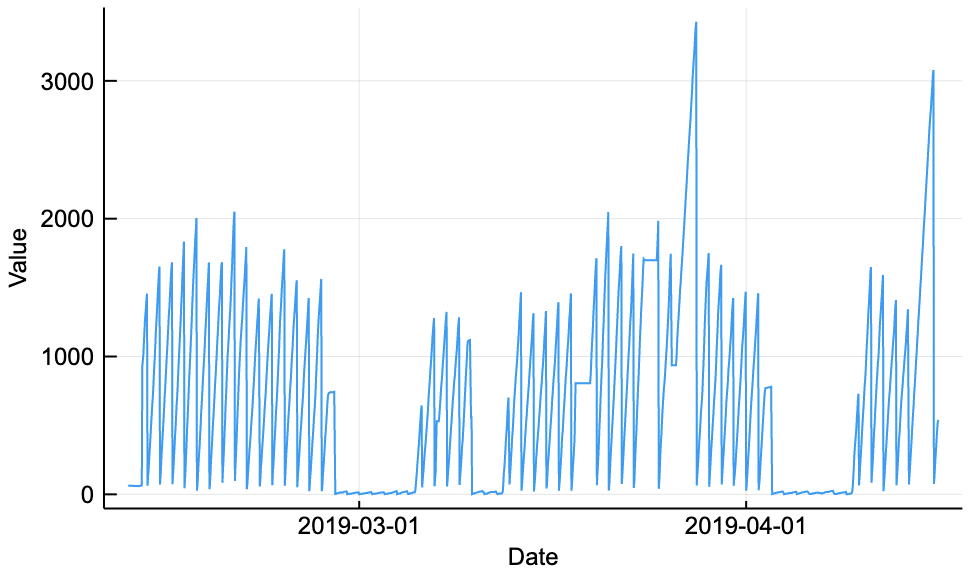
\includegraphics[width=\columnwidth]{dailymono.png} % requires the graphicx package
   \caption{Daily Monotonic Time Series}
   \label{fig:dailymono}
\end{figure}

As seen in the plot, the values in daily monotonic time series is monotonically increasing and resets to certain baseline the following day and starts to rise again until the end of the daily cycle.
\vskip 2pt
Let us now reuse the \emph{Monotonicer} filter we used in the previous subsection to normalise the data.

\begin{lstlisting}[language = Julia]
dailymonopipeline = Pipeline(Dict(
  :transformers => [dailymonocsv,valgator,
                    valputer,mononicer,pltr]))
fit!(dailymonopipeline)
transform!(dailymonopipeline)
\end{lstlisting}

\begin{figure}[htbp]
   \centering
   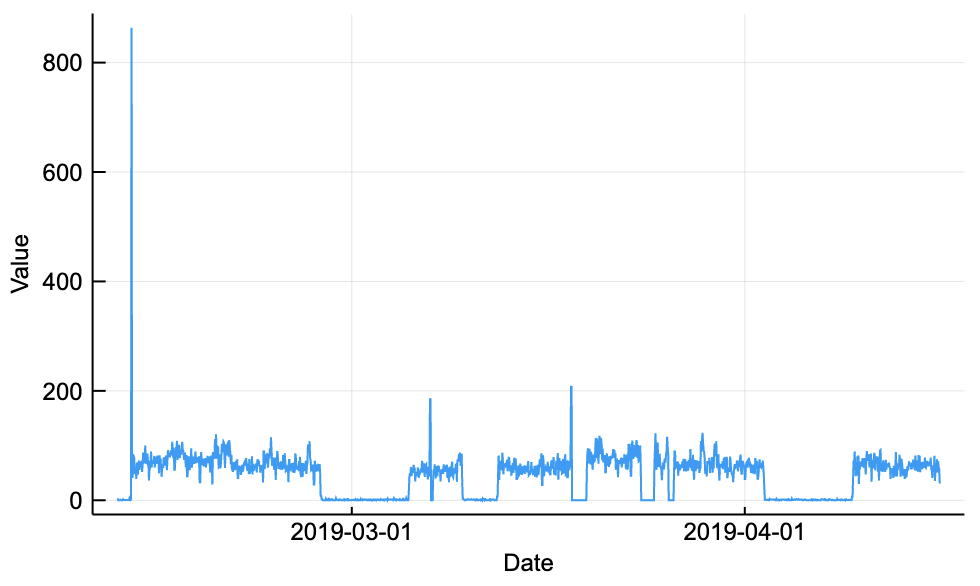
\includegraphics[width=\columnwidth]{normdailymono.png}  % requires the graphicx package
   \caption{Normalized Daily Monotonic Time Series}
   \label{fig:ndailymono}
\end{figure}

To remove outliers, we can reuse the \emph{Outliernicer} filter in the previous subsection and plot the cleaned data.

\begin{lstlisting}[language = Julia]
dailymonopipeline = Pipeline(Dict(
  :transformers=>[dailymonocsv,valgator,valputer,
                  mononicer,outliernicer,pltr]))
fit!(dailymonopipeline)
transform!(dailymonopipeline)
\end{lstlisting}

\begin{figure}[htbp]
   \centering
   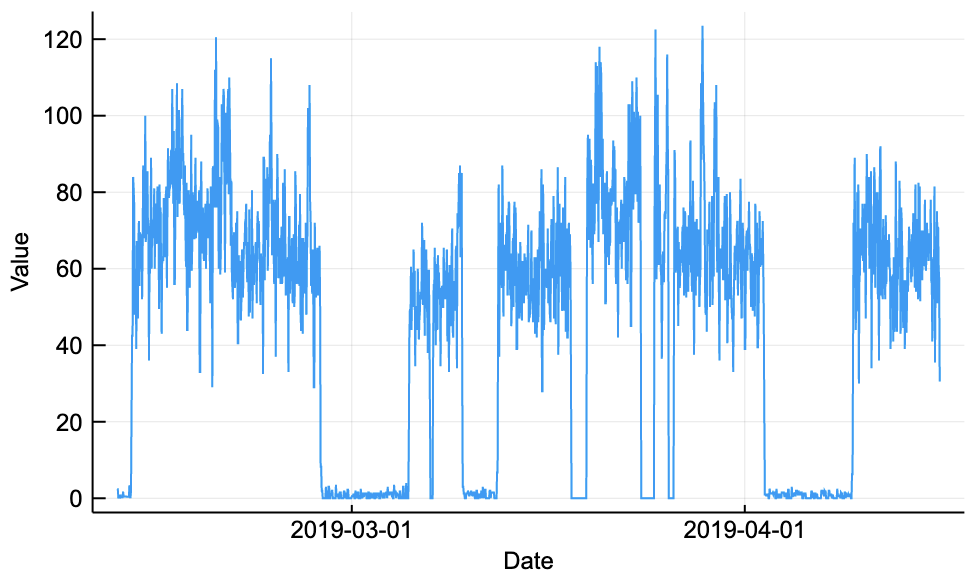
\includegraphics[width=\columnwidth]{outnormdailymono.png}  % requires the graphicx package
   \caption{Normalized Daily Monotonic Time Series with Outlier Detector}
   \label{fig:outndailymono}
\end{figure}


\section{Time Series Classification}

We can now use the knowledge we learned in setting up 
\emph{pipeline} and \emph{filters} to build higher level
operations to solve a specific industrial problem. One major problem
which we consider relevant because it is a common issue in IOT (Internet of Things) 
 is the time series classification. This problem is prevalent nowadays 
due to the increasing need to use many sensors to monitor status in different aspects of industrial
operations and maintenance of cars, buildings, hospitals, supermarkets, homes, cities, etc.

Rapid deployment of these sensors result to many of them not properly labeled or classified.
Time series classification is a significant first step for optimal prediction and anomaly detection.
To successfully perform the latter operations, it is necessary to identify first the time series
type so that appropriate model and cleaning routines can be selected for optimal model performance . 
The  \emph{TSClassifier} filter aims to address this problem and its usage is described below.

\vskip 6pt
First, we setup the locations of files for training, testing, and saving the model.
Next, we start the training phase by calling \emph{fit} which loads
file in the training directory and learn the mapping between their
statistic features extracted by \emph{Statifier} with their types indicated
by their filenames. Once the training is done, the final model
is saved in the \emph{model} directory which will be used for 
testing accuracy and classifying new time series datasets. 

The code below initialises the \emph{TSClassifier} with the locations of the training, testing, and modelling repository. Training is carried out by the \emph{fit} function which extracts the stat features of the training data and save them as a DataFrame input to the \emph{RandomForest} classifier. The trained model is saved and used during testing.

\begin{lstlisting}[language = Julia]
trdirname = joinpath(dirname(pathof(TSML)),
     "../data/realdatatsclassification/training")
tstdirname = joinpath(dirname(pathof(TSML)),
     "../data/realdatatsclassification/testing")
modeldirname = joinpath(dirname(pathof(TSML)),
     "../data/realdatatsclassification/model")
tscl = TSClassifier(Dict(
  :trdirectory=>trdirname,
  :tstdirectory=>tstdirname,
  :modeldirectory=>modeldirname,
  :num_trees=>75)
)
fit!(tscl)
predictions = transform!(tscl)
@show testingAccuracy(predictions)
\end{lstlisting}

Figure~\ref{fig:tcl} shows: a) a snapshot of the output during training and testing which extracts the statistical features of the time series; and b) the testing performance of the classifier. The training and testing data are labeled based on their sensor type for easier validation. The labels are not used as input during training. The classification workflow is purely driven by the statistical features. The prediction indicates 80\% accuracy.

\begin{figure}[htbp]
   \centering
   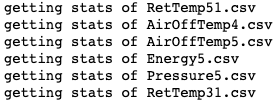
\includegraphics[width=0.5\columnwidth]{tscl1.png} % requires the graphicx package
   
   ..........
   
   ..........
   \vskip 2pt
   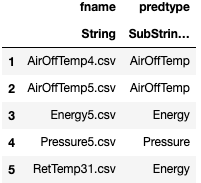
\includegraphics[width=0.4\columnwidth]{tscl2.png} % requires the graphicx package
   \caption{Extraction of Statistical Features for Training and Prediction. By convention, the \emph{TSClassifier} validates the ground truth based on the filename which contains the label of the sensor type disregarding the numerical component.}
   \label{fig:tcl}
\end{figure}

\section{Extending TSML with Scikitlearn and Caret}
In the latest \textbf{TSML} version (2.3.4 and above), 
we refactored the base TSML
to only include pure Julia code implementations and moved
external libs and binary dependencies into the TSMLextra package. 
One major reason is to have a smaller code base so that it can be easily
maintained and rapidly deployed in a dockerized solution or Kubernetes deployment. Moreover, smaller codes make
static compilation fast for smaller docker image  
in cloud deployment. 

There are cases however where the main task of time series classification 
requires more complex ensemble model using hierarchy or tree where 
members are composed of heterogeneous ML learners from binaries in 
different languages. For illustration purposes, we will show how to 
ensemble ML libraries from ScikitLearn and Caret using \textbf{TSML} 
meta-ensembles that support the \emph{fit} and \emph{transform} APIs.

\subsection{Parallel TSML Using Distributed Workflow}

We will use Julia's built-in support for parallelism by using the \emph{Distributed} library. We also let Julia detect the number of processors available and activate them.

\begin{lstlisting}[language = Julia]
using Distributed 
nprocs() == 1 && addprocs()
\end{lstlisting}

With several workers active, we can use the \emph{@everywhere} macro to load the necessary filters and transformers to all workers.

\begin{lstlisting}[language = Julia]
@everywhere using TSML
@everywhere using TSMLextra
@everywhere using DataFrames
@everywhere using Random
@everywhere using Statistics
@everywhere using StatsBase: iqr
@everywhere using RDatasets
\end{lstlisting}

With all the necessary TSML functions loaded, we can now setup the different MLs starting with some learners from Caret and ScikitLearn. The list is not exhaustive for demonstration purposes.

\begin{lstlisting}[language = Julia]
# Caret ML
@everywhere caret_svmlinear = 
   CaretLearner(Dict(:learner=>"svmLinear"))
@everywhere caret_treebag = 
   CaretLearner(Dict(:learner=>"treebag"))

# ScikitLearn ML
@everywhere sk_knn = 
  SKLearner(Dict(:learner=>"KNeighborsClassifier"))
@everywhere sk_gb = 
  SKLearner(Dict(:learner=>
    "GradientBoostingClassifier",
    :impl_args=>Dict(:n_estimators=>10)))
@everywhere sk_extratree = 
  SKLearner(Dict(:learner=>"ExtraTreesClassifier",
    :impl_args=>Dict(:n_estimators=>10)))
@everywhere sk_rf = 
  SKLearner(Dict(:learner=>
    "RandomForestClassifier",
    :impl_args=>Dict(:n_estimators=>10)))
\end{lstlisting}

Let us setup instances from thebpure Julia implementation of learners and ensembles based on the \emph{DecisionTree.jl} package.

\begin{lstlisting}[language = Julia]
# Julia ML
@everywhere jrf = RandomForest()
@everywhere jpt = PrunedTree()
@everywhere jada = Adaboost()

# Julia Ensembles
@everywhere jvote_ens=VoteEnsemble(Dict(
   :learners=>[jrf,jpt,sk_gb,sk_extratree,sk_rf]))
@everywhere jstack_ens=StackEnsemble(Dict(
   :learners=>[jrf,jpt,sk_gb,sk_extratree,sk_rf]))
@everywhere jbest_ens=BestLearner(Dict(
   :learners=>[jrf,sk_gb,sk_rf]))
@everywhere jsuper_ens=VoteEnsemble(Dict(
   :learners=>[jvote_ens,jstack_ens,
               jbest_ens,sk_rf,sk_gb]))
\end{lstlisting}

Next, we setup the pipeline for training and prediction inside the \emph{predict} function.

\begin{lstlisting}[language = Julia]
@everywhere function predict(learner,
            data,train_ind,test_ind)        
  features = convert(Matrix,data[:, 1:(end-1)])
  labels = convert(Array,data[:, end])
  # Create pipeline
  pipeline = Pipeline(
    Dict(
      :transformers => [
        OneHotEncoder(), # nominal to bits
        Imputer(), # Imputes NA values
        StandardScaler(), # normalize
        learner # Predicts labels on instances
      ]
    )
  )
  # Train
  fit!(pipeline, features[train_ind, :],
       labels[train_ind])  
  # Predict
  predictions = transform!(pipeline, 
      features[test_ind, :])
  # Assess predictions
  result = score(:accuracy, 
      labels[test_ind], predictions)
  return result
end
\end{lstlisting}

Finally, we setup the \emph{parallel model} function to run different learners distributed to different workers running in parallel relying on Julia's native support of parallelism. Take note that there are two parallelisms in the code. The first one is the distribution of task in different trials and the second one is the distribution of tasks among different models. It is interesting to note that with this relative compact function definition, the Julia language makes it easy to define a parallel task within another parallel task without any problem.

\begin{lstlisting}[language = Julia]
function parallelmodel(learners::Dict,
         data::DataFrame;trials=5)
  models=collect(keys(learners))
  ctable=@distributed (vcat) for i=1:trials
    # Split into training and test sets
    Random.seed!(3i)
    (trndx, tstndx) = holdout(size(data, 1), 0.20)
    acc=@distributed (vcat) for model in models
      res=predict(learners[model],
             data,trndx,tstndx)
      println("trial ",i,", ",model," => ",
              round(res))
      [model res i]
    end
    acc
  end
  df = ctable |> DataFrame
  rename!(df,:x1=>:model,:x2=>:acc,:x3=>:trial)
  gp=by(df,:model) do x
    DataFrame(mean=mean(x.acc),std=std(x.acc),
              n=length(x.acc)) 
  end
  sort!(gp,:mean,rev=true)
  return gp
end
\end{lstlisting}

We can now benchmark the performance of the different machine learners by creating a dictionary of workers containing instances of learners from Caret, ScikitLearn, and Julia libraries. We pass the dictionary of learners to the \texttt{parallelmodel} function for evaluation.

\begin{lstlisting}[language = Julia]
learners=Dict(
  :jvote_ens=>jvote_ens,:jstack_ens=>jstack_ens,
  :jbest_ens=>jbest_ens,:jrf=>jrf,:jada=>jada,
  :jsuper_ens=>jsuper_ens, 
  :crt_svmlinear=>caret_svmlinear,
  :crt_treebag=>caret_treebag,
  :skl_knn=>sk_knn,:skl_gb=>sk_gb,
  :skl_extratree=>sk_extratree, :sk_rf=>sk_rf
)

datadir = joinpath("tsdata/")
tsdata = extract_features_from_timeseries(datadir)
first(tsdata,5)

respar = parallelmodel(learners,tsdata;trials=3)
\end{lstlisting}

\begin{figure}[htbp]
   \centering
   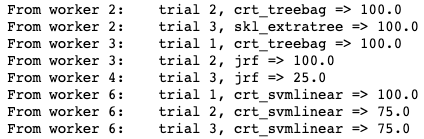
\includegraphics[width=0.8\columnwidth]{sim.png} % requires the graphicx package
   \caption{Output During Training with Several Workers}
   \label{fig:sim}
\end{figure}

\begin{figure}[htbp]
   \centering
   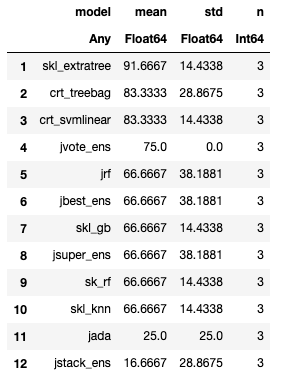
\includegraphics[width=0.6\columnwidth]{results.png} % requires the graphicx package
   \caption{@distributed: Classification Performance in 3 Trials}
   \label{fig:performance}
\end{figure}

The data used in the experiment are sample snapshots of the data in our building operations. For reproducibility, the data can be found in the  \emph{juliacon2019-paper} branch of \emph{TSML} in \emph{Github}:  /data/benchmark/tsclassifier. There are four time series types, namely: AirOffTemp, Energy, Pressure, and RetTemp.  We  took a minimal number of samples and classes for discussion and demonstration purposes.

\vskip 6pt

Figures~\ref{fig:sim}~and~\ref{fig:performance}  show a snapshot of running workers exploiting the distributed library of Julia and the classification performance of each model, respectively. There are 8 workers running in parallel over 12 different machine learning classifiers. From the results, \emph{ExtraTree} from \emph{ScikitLearn} has the best performance with 91.67\% accuracy followed by \emph{TreeBag} and \emph{SVMLinear} from \emph{Caret} library with 83.33 \% accuracy for both. With this workflow, it becomes trivial to search for optimal model by running them in parallel relying on \emph{Julia} to do the low-level tasks of scheduling, queueing, synchronizing, etc and making sure that dynamically available compute resources are fairly optimised.

\subsection{Parallel TSML Using Threads Workflow}
With Julia 1.3, lightweight multi-threading support in Julia becomes possible. We will be using pure Julia ML models because installing external dependencies such as Caret MLs through RCall package has some issues with the alpha version of Julia 1.3 at this point in time. We will update this documentation and add more MLs once the issues are resolved.

\vskip 6pt

The main difference in the workflow between Julia's distributed computation model compared to the threaded model is the presence of \texttt{@everywhere} macro in the former for each function defined to indicate that these function definitions shall be exported to all running workers. Since threaded processes share the same memory model with the Julia main process, there is no need for this macro. Instead, threading workflow requires the use of \emph{mutex} locking in the update of the global dataframe that gathers the prediction performance of models running in their respective threads. In similar observation with the distributed framework, the \emph{threadedmodel} function contains two parallelism: threads in different trials and threads among models in each trial. The function is surprisingly compact to implement threads within threads without issues and the main bottleneck happens only during the update operation of the global \emph{ctable}.

\begin{lstlisting}[language = Julia]
function threadedmodel(learners::Dict,
         data::DataFrame;trials=5)
  Random.seed!(3)
  models=collect(keys(learners))
  global ctable = DataFrame()
  @threads for i=1:trials
     # Split into training and test sets
     (train_ind, test_ind) = 
          holdout(size(data, 1), 0.20)
     mtx = SpinLock()
     @threads for themodel in models
       res=predict(learners[themodel],
          data,train_ind,test_ind)
       println(themodel," => ",round(res),", 
          thread=",threadid())
       lock(mtx)
       global ctable=vcat(ctable,
          DataFrame(model=themodel, acc=res))
       unlock(mtx)
     end
  end
    df = ctable |> DataFrame
    gp=by(df,:model) do x
       DataFrame(mean=mean(x.acc),
          std=std(x.acc),n=nrow(x))
    end
    sort!(gp,:mean,rev=true)
    return gp
end
\end{lstlisting}

Let us define a set of learners that are written in pure Julia for this thread experiment.

\begin{lstlisting}[language = Julia]
# Julia ML
jrf = RandomForest(Dict(:impl_args=>
   Dict(:num_trees=>500)))
jpt = PrunedTree()
jada = Adaboost(Dict(:impl_args=>
   Dict(:num_iterations=>20)))

## Julia Ensembles
jvote_ens=VoteEnsemble(Dict(:learners=>
   [jrf,jpt,jada]))
jstack_ens=StackEnsemble(Dict(:learners=>
   [jrf,jpt,jada]))
jbest_ens=BestLearner(Dict(:learners=>
   [jrf,jpt,jada]))
jsuper_ens=VoteEnsemble(Dict(:learners=>
   [jvote_ens,jstack_ens,jbest_ens]));
\end{lstlisting}

Let us run in parallel the different models using the same dataset with that of the distributed workflow.

\begin{lstlisting}[language = Julia]
using Base.Threads

learners=Dict(
      :jvote_ens=>jvote_ens,
      :jstack_ens=>jstack_ens,
      :jbest_ens=>jbest_ens,
      :jrf => jrf,:jada=>jada,
      :jsuper_ens=>jsuper_ens);
      
datadir = joinpath("tsdata/")
tsdata = extract_features_from_timeseries(datadir)

resthr = threadedmodel(learners,tsdata;trials=10)
\end{lstlisting}

\begin{figure}[htbp]
   \centering
   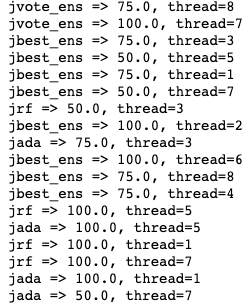
\includegraphics[width=0.5\columnwidth]{threadrunning.png} % requires the graphicx package
   \caption{Output During Training Using Several Threads}
   \label{fig:threadrunning}
\end{figure}

\begin{figure}[htbp]
   \centering
   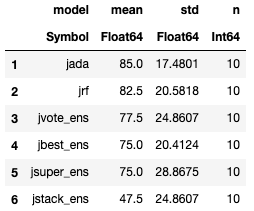
\includegraphics[width=0.5\columnwidth]{threadresult.png} % requires the graphicx package
   \caption{@threads: Classification Performance in 10 Trials}
   \label{fig:threadresult}
\end{figure}

Figures~\ref{fig:threadrunning}~and~\ref{fig:threadresult} show example snapshot of the running threads and the final result of classification, respectively. In this experiment, Adaboost has 85\% accuracy followed by Random Forest with 82.5\% accuracy.

\section{Summary and Conclusion}
Packages for time series analysis are becoming important tools with the rapid proliferation of sensor data brought about by \textbf{Internet of Things}.  We created \emph{TSML} as a time series machine learning framework which can easily be extended to handle large volume of time series data. 

\vskip 6pt

\emph{TSML} main strength is the adoption of pipeline architecture containing filters and transformers to perform both preprocessing and modelling tasks. \emph{TSML}  exploits the following \emph{Julia} features: multiple dispatch, type inference, custom data types and abstraction, and parallel computations.  In addition, \emph{TSML} uses a common machine learning API for both internal and external ML libraries, distributed and threaded support for modeling, and a growing collection of filters for preprocessing, classification, clustering, and prediction. Extending \emph{TSML} can trivially be done by creating a custom data type filter and defining its corresponding \emph{fit} and \emph{transform} operations which the \emph{TSML} pipeline iteratively calls on its collection of filters.

%TODO: 
%\begin{itemize}
%\item add threading examples for scalability (buggy, need fixes)
%\item add simulations of different datasets to show general applicability (still doing simulations): %Earthquakes sensor; Electric Devices; car sensors; refrigeration devices; household consumption
%\end{itemize}

% **************GENERATED FILE, DO NOT EDIT**************

\bibliographystyle{juliacon}
\bibliography{ref.bib}


\end{document}

% Inspired by the International Journal of Computer Applications template
